%%%%%%%%%%%%%%%%%%%%%%%%%%%%%%%%%%%%%%%%%
% fphw Assignment
% LaTeX Template
% Version 1.0 (27/04/2019)
%
% This template originates from:
% https://www.LaTeXTemplates.com
%
% Authors:
% Class by Felipe Portales-Oliva (f.portales.oliva@gmail.com) with template 
% content and modifications by Vel (vel@LaTeXTemplates.com)
%
% Template (this file) License:
% CC BY-NC-SA 3.0 (http://creativecommons.org/licenses/by-nc-sa/3.0/)
%
%%%%%%%%%%%%%%%%%%%%%%%%%%%%%%%%%%%%%%%%%

%----------------------------------------------------------------------------------------
%	PACKAGES AND OTHER DOCUMENT CONFIGURATIONS
%----------------------------------------------------------------------------------------

\documentclass[
  french,
  % twocolumn,
	11pt, % Default font size, values between 10pt-12pt are allowed
	%letterpaper, % Uncomment for US letter paper size
	%spanish, % Uncomment for Spanish
]{fphw}

% \usepackage[fontsize=10.0]{scrextend} % Use this to force the fontsize

%% Commands for numbering paragraphs
\renewcommand\thesection{\Roman{section}}
\renewcommand\thesubsection{\thesection.\arabic{subsection}}
\renewcommand*\thesubsubsection{%
  \Roman{section}.\arabic{subsection}.\alph{subsubsection}%
}

\usepackage{sectsty}
\sectionfont{\sf\bfseries\LARGE\raggedright}

% Template-specific packages
% \usepackage{babel}


% \renewcommand*\familydefault{\sfdefault}
\usepackage[utf8]{inputenc} % Required for inputting international characters
% \usepackage{DejaVuSerifCondensed} 
\usepackage[T1]{fontenc} % Output font encoding for international characters
\usepackage{textcomp}

\usepackage[lf]{venturis}
% \usepackage[libertine]{newtxmath}
\usepackage{libertinust1math}
\usepackage{bm} 

\usepackage{fancyvrb}
\usepackage{fvextra}
\newcommand\userinput[1]{\textbf{#1}}
\newcommand\arguments[1]{\textit{#1}}

\usepackage{amsmath}
\usepackage{mathtools}
\usepackage{xfrac} 
% \usepackage{amssymb}
% \usepackage{enumitem}	%% % To modify the itemize bullet character 

\usepackage{graphicx} % Required for including images
\usepackage[textfont=it,font=small]{caption}  %% To manage long captions in images
\usepackage{subcaption}
\captionsetup{justification=centering}

\usepackage{float}
\graphicspath{ {../img/} }

\usepackage{booktabs} % Required for better horizontal rules in tables

\usepackage{listings} % Required for insertion of code

\usepackage{array} % Required for spacing in tabular environment

\usepackage{enumerate} % To modify the enumerate environment

\newcommand{\tabhead}[1]{{\bfseries#1}}

\usepackage{xcolor}
\usepackage{listings}
\colorlet{mygray}{black!30}
\colorlet{mygreen}{green!60!blue}
\colorlet{mymauve}{red!60!blue}

\usepackage[linkcolor=blue,colorlinks=true]{hyperref}
% \usepackage[colorlinks=true,urlcolor=blue]{hyperref}
\hypersetup{citecolor=blue}

\usepackage{cleveref}
\usepackage{siunitx}

\usepackage[backend=bibtex,style=alphabetic,maxnames=2,natbib=true]{biblatex} % Use the bibtex backend with the alphabetic citation style (compact APA-like)
% \usepackage[backend=bibtex,style=authoryear,maxnames=2,natbib=true]{biblatex} % Use the bibtex backend with the authoryear citation style (which resembles APA)
\addbibresource{bibliography.bib} % The filename of the bibliography
\usepackage[autostyle=true]{csquotes} % Required to generate language-dependent quotes in the bibliography 
% \renewcommand*{\bibfont}{\tiny} % Pour reduire la taille des references

\usepackage[useregional=numeric]{datetime2}
\usepackage[normalem]{ulem}

% %-------------------------------------------------------------------------------

\newcommand{\myvec}[3]{\begin{pmatrix} #1  \\ #2 \\ #3 \end{pmatrix}}   %% vecteur 3d
\newcommand{\mymat}[9]{\begin{pmatrix} #1 & #2 & #3 \\ #4 & #5 & #6 \\ #7 & #8 &#9 \end{pmatrix}}  %% Matrice 3*3

\renewcommand{\vector}[4]{\begin{pmatrix} #1  \\ #2 \\ #3 \\ #4 \end{pmatrix}}   %% vecteur 4d
% \newcommand{\mymatrix}[16]{\begin{pmatrix} #1 & #2 & #3 & #4 \\ #4 & #6 & #7 & #8 \\ #9 & #10 & #11 & #12 \\ #13 & #14 & #15 & #16 \end{pmatrix}}  %% Matrice 3*3

\newcommand{\hquad}{\hspace{0.5em}} %% Bew command for half quad
\newcommand*\diff{\mathop{}\!\mathrm{d}}
% \setlength\parindent{0pt}	%% To remove all indentations
\newcommand{\bvec}[1]{\bm{\mathrm{#1}}}  %% Use this to make vectors
\newcommand{\bmat}[1]{\bm{\mathsf{#1}}}   %% Use this to make tensors


%----------------------------------------------------------------------------------------
%	ASSIGNMENT INFORMATION
%----------------------------------------------------------------------------------------

\title{\sf\bfseries Compte rendu semaine \#19} % Assignment title
% \title{Difficultés rencontrées} % Assignment title

\author{Roussel Desmond Nzoyem} % Student name 

\date{\DTMdisplaydate{2021}{6}{09}{-1} - \DTMdisplaydate{2021}{6}{15}{-1}} % Due date

\institute{Sorbonne Université \\ Laboratoire Jacques-Louis Lions} % Institute or school name

\class{Stage M2} % Course or class name

\professor{Pr. Stéphane Labbé} % Professor or teacher in charge of the assignment

%----------------------------------------------------------------------------------------

\begin{document}

\maketitle % Output the assignment title, created automatically using the information in the custom commands above

%----------------------------------------------------------------------------------------
%	ASSIGNMENT CONTENT - INTRO
%----------------------------------------------------------------------------------------

Le point marquant de cette semaine fut l'étude approfondie du problème de percussion 1D. J'ai en effet simulé le phénomène de percussion en présences de floes ayant deux ou plusieurs noeuds chacun. J'ai aussi effectué une étude énergétique des systèmes après m'être rassuré sur le coefficient de restitution.

%----------------------------------------------------------------------------------------
%	ASSIGNMENT CONTENT - SECTION 1
%----------------------------------------------------------------------------------------

\section*{Tâches effectuées}


\begin{enumerate}
  \item Implémentation du module \href{https://github.com/desmond-rn/ice-floes/blob/master/code/simu1D/Modules/Solveur1D.py}{Solveur1D.py} pour la simulation de la percussion.
  \item Migration du code préexistant (depuis les notebook Python) vers le module \texttt{Solveur1D.py} lorsque possible afin d'accélérer le travail.
  \item Étude du coefficient de restitution utilisé en mécanique du contact (voir \parencite[p.21]{acary2004coefficients} ainsi que l'email du dimanche 13 juin dernier).
  \item Étude énergétique pour la validation du système. On peut par exemple voir un des résultats à la \cref{fig:myfig}. L'animation des floes correspondants est donnée en pièce jointe.
  \begin{figure}[H]
    \centering
    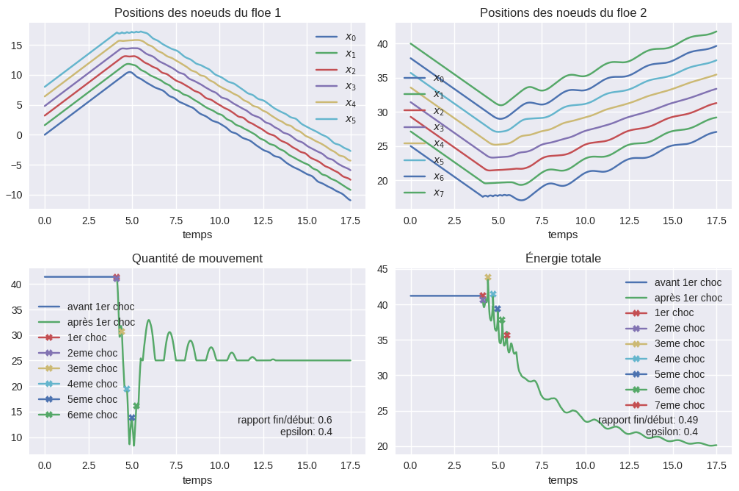
\includegraphics[width=0.78\textwidth]{Plots1D.png}
    \caption{Plots de quelques quantités dans le problème de percussion 1D. Les paramètres physiques du problème sont: $m = 1.5, \, m' = 1.5,\, k = 80,\, k' = 70,\, \mu = 0.0,\, \mu' = 2.0,\, v_0 = 2.2,\, v'_0 = -1.8,\, \varepsilon  = 0.4$}
    \label{fig:myfig}
  \end{figure}
\end{enumerate}


 
%----------------------------------------------------------------------------------------
%	ASSIGNMENT CONTENT - SECTION 2
%----------------------------------------------------------------------------------------

\section*{Difficultés rencontrées}


\begin{enumerate}
  \item La première difficulté fut dans la simulation de la percussion avec plusieurs noeuds. En plus de considérer un nombre indéfini de noeuds par floes, ce nouveau travail observe et traite plusieurs collisions (contrairement au travail précédent qui ne traitait qu'une seule). Sur ce point, nous nous somme encore mieux rapproché de la notion de \emph{percussion}. 
  \item La deuxième est dans l'étude de la quantité de mouvement et de l'énergie totale du système. Comme on peut l'observer à la \cref{fig:myfig}, il n'y a pas conservation de l'énergie totale du système. Je suspecte que c'est dû à la formule de calcul de l'énergie dissipée par les frottements visqueux, qui d'après les travaux de Dimitri, vaut :
  \begin{figure}[H]
    \centering
    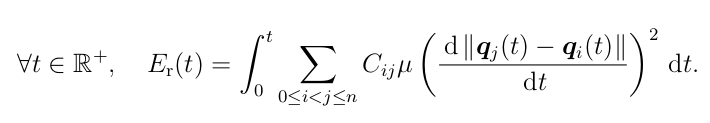
\includegraphics[width=0.78\textwidth]{EnergieDissipee.png}
    \caption{Formule de l'énergie dissipée par frottement visqueux \parencite[p.188]{balasoiu2020halthesis}.}
    \label{fig:myfig2}
  \end{figure}
\end{enumerate}



%----------------------------------------------------------------------------------------
%	ASSIGNMENT CONTENT - SECTION 3
% ----------------------------------------------------------------------------------------
\section*{Travail à venir}

\emph{Par ordre de priorité :}

\begin{enumerate}
  \item Révision de l'étude énergétique pour avoir la conservation voulue.
  \item Étude de la possibilité de faire des expériences en laboratoire pour valider (ou invalider) le modèle.
  \item Écriture du modèle de percussion avec plusieurs noeuds (ainsi que les résultats) dans le rapport de stage.
  \item En cas de réussite des trois premières tâches ci-haut, que faire par la suite ? Faut-il implémenter un nouveau modèle 2D basé sur ce modèle 1D, ou faut-il se baser sur celui de Dimitri ?
\end{enumerate}



 
% %-------------------------------------------------------------------------------
% %							THE BIBLIOGRAPHY
% %-------------------------------------------------------------------------------
\clearpage   % Pour retirer les references de la bare de navigation
\printbibliography


\end{document}
